\documentclass[journal,12pt,twocolumn]{IEEEtran}

\usepackage{amsmath}
\usepackage{amssymb}
\usepackage{amsthm}
\usepackage{graphicx}
\usepackage{gensymb}


\parindent 0px


\vspace{3cm}
\title{ Assignment 1}

\author{\textbf{\textit{Sri Charvi}}\\
\textbf{\textit{BT21BTECH11008}}}


\begin{document}

\maketitle
\textbf{Q10(b) }: A man observes the angle of elevation of the top of the tower to be 45º.
 He walks towards it in a horizontal line through its base. On covering 20 m the angle of 
elevation changes to 60º. Find the height of the tower correct to 2 significant figures.\\

\medskip
\textbf{Solution}: Let the height of the tower be `$h$' and total distance between man and the tower be `$d$'.\\

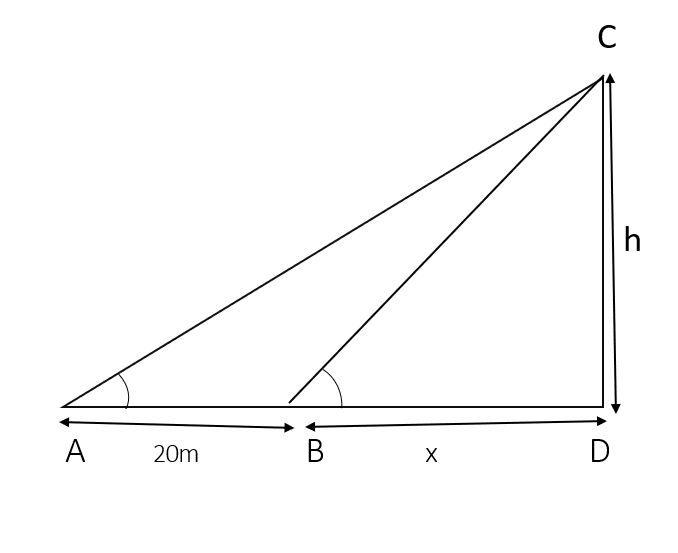
\includegraphics[scale=0.4]{Fig1}\\
Given that, $ \angle CAD=45\degree \text{ and } \angle CBD=60\degree.$ Let the given angles
be $\theta_1=45\degree \text{ and } \theta_2=60\degree.$

From the given information,
\begin{align}
d=20+x\\
hcot\theta_1=d\\
hcot\theta_2=x
\end{align}
Solving the equations (1),(2),(3),we get
\begin{align*}
 hcot\theta_1&=20+hcot\theta_2\\
 h&=\frac{20}{cot\theta_1-cot\theta_2}\\
 h&=\dfrac{20}{\left(1-\frac{1}{\sqrt{3}}\right)}\\
 h &= 47.32m
\end{align*}

$\therefore $ The height of the tower is 47.32 m






\end{document}